\section{The Privacy Dilemma and UPPRESSO Overview}
%\section{The Identifier-Transformation Approach of UPPRESSO}
\label{sec:challenge}
Next, we overview the required security and privacy properties of an SSO system. Then, we conceptualize the SSO privacy problem as an identifier-transformation problem and explain the privacy dilemma behind existing solutions. Finally, we present the design goals of UPPRESSO. %'s identifier-transformation framework.
We list the notations used in the discussion in Table~\ref{tbl:notations} for reference.

\subsection{Security Properties of SSO}
\label{subsec:basicrequirements}
The primary goal of SSO services is to support secure user authentication~\cite{SPRESSO}, which ensures that a legitimate user can always log in to (her unique account at) an honest RP. To achieve this, the identity proof generated by the IdP should explicitly specify the user who is authenticated by the IdP (i.e., \textbf{\textit{user identification}}) and the RP to which the user requests to log in (i.e., \textbf{\textit{RP designation}}). To provide continuous service, the user identification property also requires an RP to be able to recognize a user and correlate her multiple logins by her unique identifier or account. Moreover, the identify proof generated by the IdP should be transmitted only to the dedicated RP (directly or through the user) (i.e., \textbf{\textit{confidentiality}}) and should not be modified or forged (i.e., \textbf{\textit{integrity}}). We summarize these four security properties from theoretical analysis of SSO designs~\cite{ArmandoCCCT08,FettKS16, FettKS17} and practical attacks~\cite{SomorovskyMSKJ12, WangCW12, ArmandoCCCPS13, ZhouE14, WangZLLYLG15, WangZLG16, YangLLZH16, MainkaMS16, MainkaMSW17, YangLCZ18, YangLS17, ShiWL19, ChenPCTKT14, ccsSunB12, DiscoveringJCS, dimvaLiM16, CaoSBKVC14, TowardsShehabM14}.

Many attacks exploit vulnerabilities in SSO design and implementation to break at least one of the four security properties. %~\cite{ChenPCTKT14, FettKS16,WangCW12,ZhouE14,WangZLG16,YangLLZH16,SomorovskyMSKJ12,MohsenS16}.
The adversary mainly aims to log in to an honest RP as a victim user (called \emph{impersonation attacks}) or allure a victim user to log in to an honest RP under the attacker's account (called \emph{identity injection attacks}). For example, Friendcaster used to accept every received identity proof (i.e., a violation of RP designation)~\cite{ChenPCTKT14}. So, a malicious RP can replay a received identity proof to Friendcaster and log in as the victim user. If identity proofs are leaked (i.e., a violation of confidentiality)~\cite{WangCW12,ccsSunB12,ArmandoCCCPS13,DiscoveringJCS,dimvaLiM16}, the adversary can directly impersonate the victim user.
It was also reported that some RPs of Google ID SSO accepted user attributes that were not tied to the identity proofs (i.e., a violation of integrity)~\cite{WangCW12}, so that an adversary can insert arbitrary attributes (e.g., email of the adversary or another user) into the identity proof of the victim user. %to impersonate another user at the RP.

\begin{table}[tb]
\scriptsize
    \caption{The notations used in UPPRESSO.}
    \centering
%    \begin{tabular}{|c|c|c|}
    \setlength{\tabcolsep}{1.2mm}
    \begin{tabular}{|p{1.12cm}|p{4.65cm}|p{1.7cm}|}
    \hline
    {\textbf{Notation}} & {\textbf{Definition}} & {\textbf{Attribute}} \\
    \hline
    {$q$} & {A large prime, the size of the underlying field.} & {Long-term} \\
    \hline
    {$E$}&{An elliptic curve defined over a finite field $\mathbb{F}_q$ ($P-256$).}&{Long-term}
     \\
    \hline
    {G}&{A point in $E(\mathbb{F}_q)$,  known as the base point.}&{Long-term}\\
    \hline
    {$n$} & {the order of the base point $G$.} & {Long-term} \\
    \hline
%    {$L$} & {Length of $q$. } & {Long-term} \\    \hline
 %    {$g$} & {A generator of order $q$ in $GF(p)$. } & {Long-term constant} \\
    % \hline
   % \hline
    %{$SK_{ID}$, $PK$} & {The private/public key to sign/verify identity proof.} & {System-unique} \\
    {$SK$, $PK$} & {The private/public key of IdP. } & {Long-term} \\
    \hline
   {$ID_{RP}$} & {An RP's unique identity,  a point in cyclic subgroup of $E(\mathbb{F}_q)$ generated by $P$.} & {Long-term} \\
    \hline
%    {$r$} & {value for $ID_{RP}=g^r \bmod p$.} & {Secret, Long-term} \\
%    \hline
    {$Cert_{RP}$} & {An RP certificate, containing the RP's identity and endpoint.} & {Long-term} \\
    \hline
    {$ID_U$} & {A user's unique identity.} & {Long-term} \\
    \hline
     {$Account$} & {A user's identifier at an RP: $A=  {ID_U}{ID_{RP}} $ (denoted as $A$ in equations).} & {Long-term} \\
    \hline
    {$PID_{RP}$} & {$PID_{RP} = {N_{U}}{ID_{RP}} $, an RP's pseudo-identifier.} & {One-time} \\
    \hline
    {$PID_U$} & {$PID_U = {ID_U}{PID_{RP}}$, a user's pseudo-identifier.} & {One-time}\\
    \hline
    {$N_U$} & {A user-generated nonce for $PID_{RP}$.} & {One-time} \\
    \hline
 %   {$N_{RP}$} & {An RP-generated nonce for $PID_{RP}$.} & {One-time variable} \\
  %  \hline
   % {$Y_{RP}$} & {$Y_{RP} = {ID_{RP}}^{N_{RP}} \bmod p$, the public value for $N_{RP}$.} & {One-time variable} \\
    %\hline
    {$T$} & {The trapdoor to derive $Account$: $T=N_U^{-1} \bmod n$.} & {One-time} \\
    \hline
    \end{tabular}
    \label{tbl:notations}
    \vspace{-5mm}
\end{table}


\begin{comment}
We summarize the basic requirements of SSO systems based on existing theoretical analyses~\cite{ArmandoCCCT08,FettKS16, FettKS17} and practical attacks~\cite{SomorovskyMSKJ12,WangCW12,ArmandoCCCPS13,ZhouE14,WangZLLYLG15,WangZLG16,YangLLZH16,MainkaMS16,MohsenS16,MainkaMSW17,YangLCZ18,YangLS17,ShiWL19}. These requirements enable an SSO system to provide qualified authentication services for RPs, through identity proofs.
\begin{itemize}
\item \textbf{User identification.} When a user logs into a certain RP for multiple times by submitting identity proofs, the RP extracts the identical user identifier from these identity proofs, to provide personalized services for this user.
\item \textbf{RP designation.} The designated receiver (or RP) is specified in an identity proof, so that this identity proof is accepted by the visited RP only.
\item \textbf{Integrity and confidentiality.} Only the IdP is trusted to generate identity proofs, RPs do not accept an identity proof with any modification or a forged one. %RPs should only accept the valid identity proof.
Meanwhile, a valid identity proof is transmitted only to the user and the designated RP. % confidentiality of the identity proof is ensured during the transmission among the IdP, user and the designated RP.
\end{itemize}

%These basic requirements are the minimum properties that an SSO system has to provide.
% therefore RPs should be able to identify the user with the help from IdP.
First of all, user identification is necessary for common SSO systems to help the RPs to receive the user's identifier, except the anonymous services.
Any violation of these requirements \cite{SomorovskyMSKJ12,WangCW12,ArmandoCCCPS13,ZhouE14,WangZLLYLG15,WangZLG16,YangLLZH16,MainkaMS16,MohsenS16,MainkaMSW17,YangLCZ18,YangLS17,ShiWL19} result in \emph{impersonation attacks} (i.e., the adversaries log into an honest RP as a victim user) or \emph{identity injection attacks} (i.e., a victim user logs into an honest RP under some attacker's identity).
% and without integrity, the impersonation and identity injection attacks could be constructed easily
% as an adversary could directly modify user's identifier in the identity proof;
If the designated RP is not well specified or verified in identity proofs, the adversaries could deceive an RP to accept the identity proofs generated for other RPs, so that the adversaries would (\emph{a}) impersonate some victim user, by colluding with a malicious RP to obtain such an identity proof and submitting it to the RP, or (\emph{b}) inject such identity proofs in the communications between the victim user and some RP.
   %                  for example, by CSRF~\cite{zeller2008cross}.
Impersonation and identity injection attacks would be successfully launched, if the attackers could arbitrarily modify the user identifiers in identity proofs.
Or, the adversaries could impersonate the victim user by submitting any leaked identity proof to the RP~\cite{ChenPCTKT14,FettKS16,WangZLG16}, if confidentiality is not well ensured.

The design and implementation of a secure SSO system is challenging, while various vulnerabilities have been found and exploited to break at least one requirement~\cite{ChenPCTKT14, FettKS16,WangCW12,ZhouE14,WangZLG16,YangLLZH16,SomorovskyMSKJ12,MohsenS16}.
For example, Friendcaster was found to accept any received identity proof~\cite{ExplicatingSDK,ChenPCTKT14}
(i.e., a violation of RP designation) so that a malicious RP could log into Friendcaster as the victim user by replaying the identity proof received from the user to Friendcaster~\cite{MohsenS16}. \cite{WangCW12} reported that some RPs of Google ID SSO accepted user attributes that were not tied to the identity proof (i.e., a violation of integrity). As a result, a malicious user could insert arbitrary attributes (e.g., an email address) into the identity proof to impersonate another user at the RP.
\end{comment}


%\subsection{The Identity Dilemma of Privacy-Preserving SSO}
\subsection{The Privacy Dilemma in SSO Identity Proofs}
\label{subsec:challenges}

%As discussed in Section \ref{sec:intro}, existing SSO systems are vulnerable to IdP-based login tracing and RP-based identity linkage privacy leakage.
A secure SSO system should have {\em all} four security properties discussed above while preventing IdP-based login tracing and RP-based identity linkage privacy leakage. However, meeting the security and privacy requirements at the same time incurs a dilemma in the generation of identity proofs.
%Since integrity and confidentiality are ensured by digital signatures of the IdP and TLS communications in the system \cite{OpenIDConnect}, we focus only \emph{user identification} and \emph{RP designation} in the remainder.

An identity proof contains identities/identifiers of a user and an RP, which is to tell the RP that this user has been authenticated by the IdP.
% Let us denote the long-term unique identifiers of the user and the RP as $ID_U$ and $ID_{RP}$, respectively.
Since the IdP always knows the user's identity (i.e., $ID_U$), to prevent IdP-based login tracing, we should not reveal the RP's long-term identity (i.e., $ID_{RP}$) to the IdP. This leaves us no option but to use a transitional pseudo-identifier (denoted as $PID_{RP}$) to hide the real $ID_{RP}$. To ensure RP designation, $PID_{RP}$ should be uniquely associated with the RP in the identity proof request, while an RP should use different $PID_{RP}$s in different login instances. $PID_{RP}$ can be generated by the user, the RP, or together. But it should be computationally infeasible for the IdP to derive the $ID_{RP}$ from a $PID_{RP}$.

Meanwhile, to prevent RP-based identity linkage, the IdP should not directly include $ID_U$ in the identity proof. So, the IdP has to generate a transitional pseudo-identifier for the user (denoted as $PID_U$) and bind it to the identity proof. While $PID_U$ should not disclose any information for the RP to derive $ID_U$, it should also allow the RP to distinguish one user from other users. This means, to ensure user identification, an RP should be able to correlate one user's different $PID_U$s in different login instances, for example, by linking them to the same unique user account, as the RP recognizes a user by her user account (denoted as $Account$). However, collusive RPs should not be able to correlate one user's $Account$s at different RPs or infer some accounts belong to the same user.
%the requesting RP should be able to recognize and associate $PID_U$ to her unique account at the RP (denoted as $Account$). Similarly, it should be computationally infeasible for the RP to derive $ID_{U}$ from $PID_{U}$ or $Account$.

We illustrate the relationships among the identities, pseudo-identifiers and the identity proofs in Figure~\ref{fig:IDCorrelation}. The red and green blocks represent long-term identities and one-time pseudo-identifiers, respectively. The arrows denote how the pseudo-identifiers are obtained. To protect user privacy, the identity proof should use only one-time pseudo-identifiers and $PID_U$ and $PID_{RP}$ should satisfy the above requirements. This causes a \textbf{\em privacy dilemma} for the IdP: given a user ($ID_U$) and an unknown RP ($PID_{RP}$), the IdP is expected to generate a pseudo-identifier ($PID_{U}$), which is correlated with a long-term account that uniquely identifies the user at that RP, {\em without knowing anything about the RP's identity nor the user account at the RP}.
%however, the IdP is assumed to know nothing about the RP's identity nor the user account at the RP.

To solve the dilemma, we should provide the IdP some information related to the user's $Account$ at the RP to assist the generation of $PID_U$, so that $PID_U$ can be correctly correlated with the $Account$. Meanwhile, such information should not provide any additional knowledge for the IdP to derive the RP's identity, or for two RPs to correlate two $Account$s belonging to the same user. Therefore, the privacy protection problem can be converted into an identifier-transformation problem, which aims to design three identifier-transformation functions $\mathcal{F}_{ID_{U} \mapsto PID_U}$, $\mathcal{F}_{ID_{RP} \mapsto PID_{RP}}$, and $\mathcal{F}_{PID_{U} \mapsto Account}$ to compute $PID_U$, $PID_{RP}$, and $Account$, which have the above desired properties.

\begin{figure}
  \centering
  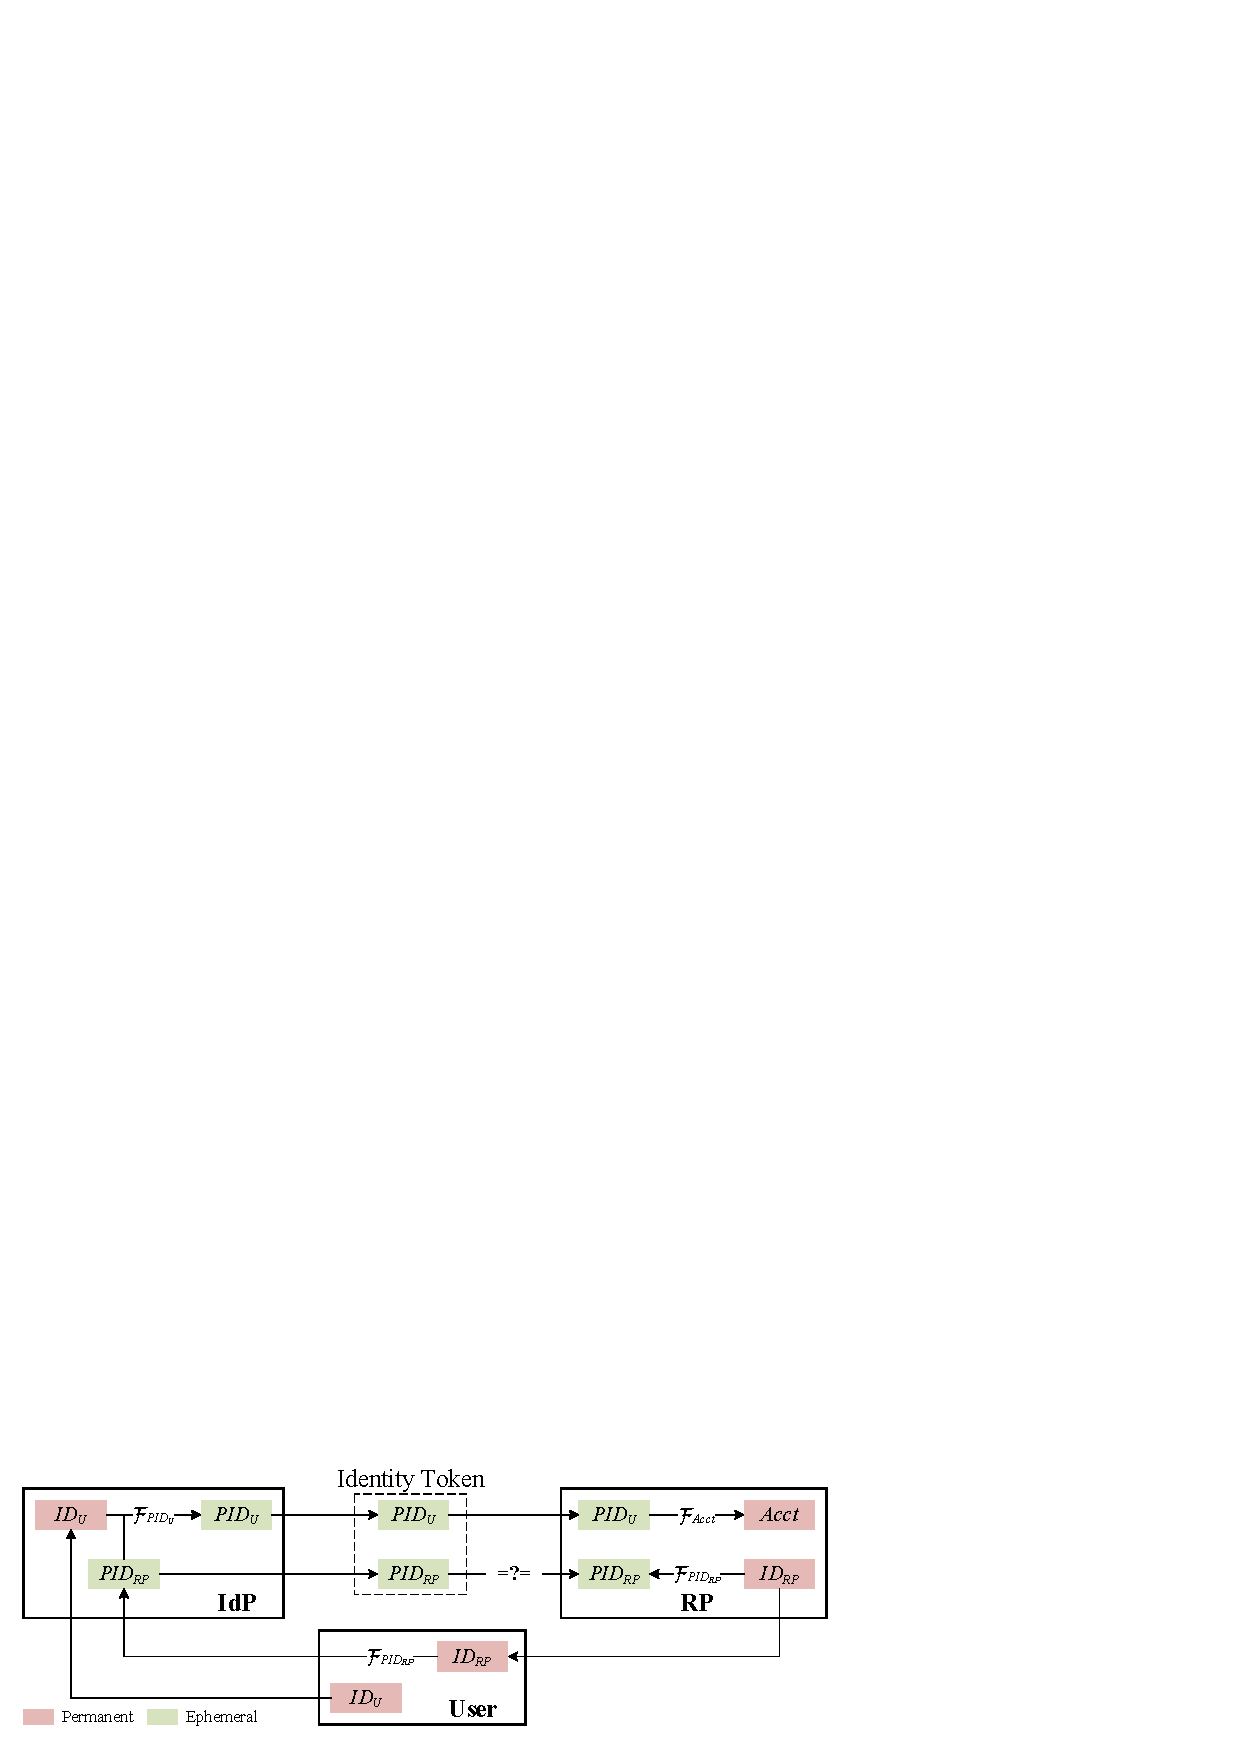
\includegraphics[width=\linewidth]{fig/IDCorrelation.pdf}
  \caption{Identifier transformations in privacy-preserving SSO.}
  \label{fig:IDCorrelation}
  \vspace{-5mm}
\end{figure}


\subsection{The Identifier-Transformation Framework of UPPRESSO}
\label{subsec:solutions}

To achieve this goal, UPPRESSO constructs three transformation functions in an integrated way to support {\em transformed RP designation} and {\em trapdoor user identification}, where (a) different $PID_U$s and $PID_{RP}$s are dynamically generated in different logins; (b) in each login session, $PID_{RP}$ is used to assist the generation of $PID_U$, which helps to link $PID_U$ to $Account$ using the trapdoor of this login session.%; and (c) when a user logs in to an RP multiple times, the RP can correlate each pair of $PID_U$ and $PID_{RP} with an invariant $Account$.


\begin{comment}
three pseudo-identifiers (i.e., $PID_U$, $PID_{RP}$, and $Account$)
in a \emph{dynamical} and \emph{comprehensive} way,
    based on \emph{static} $ID_U$ and $ID_{RP}$.
% user和RP,协商trapdoor,给$PID_U$, $PID_{RP}$带进来随机因子,同时使得只有trapdoor的RP能够计算得到Account。
That is,
    for a certain user,
in each login process at an RP,
    $PID_U$ and $PID_{RP}$ vary
        to satisfy the requirements of privacy;
but $PID_U$ and $PID_{RP}$ vary synchronously so that identical $Account$s are derived.
In particular,
    the user and the RP negotiate $PID_{RP}$ based on $ID_{RP}$ in each login process,
        and then $PID_{RP}$ is transmitted by the user to the IdP.
        Then, the IdP generates $PID_U$ based on $ID_U$ and also $PID_{RP}$.
At the same time, the RP obtains a private trapdoor in the negotiation,
    which is used to derive $Account$ from $PID_U$.

\end{comment}


%Then, we analyze the generation and use of $PID_U$ and $PID_{RP}$, considering the basic requirements of SSO system.
%\begin{itemize}
%%  \item %What's the requirement considering $PID_{U}$ and $PID_{RP}$ together? $PID_{U}$ and $PID_{RP}$一起考虑时需要满足的。
%%  The generation of $PID_{U}$ and $PID_{RP}$ must ensure the \textbf{user identification},
%%  that is, the RP could derive a same $Account$ with the $PID_{U}$ and $PID_{RP}$ from different logins. We assume RP calculates $Account$ by invoking $\mathcal{F}_{PID_{U} \mapsto Account}$ with $PID_U$, $ID_{RP}$ and $PID_{RP}$.
%
%  \item %Who generates $PID_{RP}$, and what's the requirement? PID_RP可以由RP或者user合作生成,但要保证唯一性。
%  Each $PID_{RP}$ must be globally unique, i.e., only assigned to one RP,  for achieving the \textbf{RP designation}.
%        The user and RP may generate the $PID_{RP}$ separately or cooperatively, through the function $\mathcal{F}_{ID_{RP} \mapsto PID_{RP}}$.
%        However, both the user and RP must check the uniqueness of $PID_{RP}$ before accept and use it.
%        If either the user or the RP doesn't perform the check, the adversary could make it accept a $PID_{RP}$ same as an RP and then misuse the identity proof.
%        %$PID_{RP}$ is one form of the RP's identifer, and seems unrelated with the user's identifier.
%        %Although, the user may inject the user's information into $PID_{RP}$, these information will be treated as random values at the RP and never be used to calculate $Account$, as the user is not trusted by the RP.
%        %Therefore, we can assume that $PID_{RP}$ is generated through $\mathcal{F}_{ID_{RP} \mapsto PID_{RP}}$ with the parameter $ID_{RP}$.~\footnote{The $PID_{RP}$ may also be related with the previous $PID_{RP}$. We omit the previous $PID_{RP}$ in the parameters as it is also a transformation of $ID_{RP}$.}
%  \item The \textbf{RP designation} further requires that  $PID_{U}$ is bound with either a non-null $PID_{RP}$ or $ID_{RP}$ in identity proof.
%        When $PID_{RP}$  is non-null, IdP builds the identity proof separately and the \textbf{integrity} is also ensured.
%        When $PID_{RP}$  is null, only the user could bind $PID_{U}$ with an RP identifier (i.e., $ID_{RP}$) which is unique and checkable to the RP.
%        In this case, the user who performs the binding, must have a publicly verifiable grant from the IdP, as required by \textbf{integrity}.
%%        The binding and integrity cloud be achieved by existing public key infrastructure.
%   \item The \textbf{RP designation} also requires the identity proof will only be sent to the correct RP.
%       As IdP doesn't know $ID_{RP}$, the user or a third party trusted by the correct RP will ensure this.
%\end{itemize}


\vspace{0.5mm}
\noindent \textbf{Transformed RP designation.} To prevent IdP-based login tracing, the RP includes a $PID_{RP}$ dynamically transformed from $ID_{RP}$ in the identity proof request. UPPRESSO designs a novel trapdoor-based transformation function $\mathcal{F}_{ID_{RP} \mapsto PID_{RP}}(ID_{RP}, T)$ to compute $PID_{RP}$ based on $ID_{RP}$ and a random trapdoor $T$ that is dynamically negotiated between the user and the RP in each login. Then, the user assists the RP to register $PID_{RP}$ at the IdP through OIDC dynamic registration. When an RP receives an identity proof, it verifies if the enclosed $PID_{RP}$ is transformed from its $ID_{RP}$ and the trapdoor of this session.

%To bind dynamic $PID_{RP}$ in identity proofs signed by the IdP, the user firstly cooperates with the RP to generate $PID_{RP}$ based on $ID_{RP}$ and then registers this transformed RP identifier (i.e., $PID_{RP}$) in the IdP.
%The identifier transformation of RP is completely kept secret to the IdP. Then, the one-time $PID_{RP}$ is bound with $PID_U$ in the identity proof. $PID_{RP}$ is calculated based on $ID_{RP}$ and the trapdoor, so that the RP holding the trapdoor is able to verify the specified receiver of identity proofs with transformed $PID_{RP}$ but not $ID_{RP}$.


%\vspace{1mm}
\noindent \textbf{Trapdoor user identification.} To prevent RP-based identity linkage, we design a transformation function $\mathcal{F}_{ID_{U} \mapsto PID_U}(ID_U, PID_{RP})$ for the IdP to generate $PID_U$. When an RP receives an identity proof, another transformation function $\mathcal{F}_{PID_{U} \mapsto Account}(PID_U, PID_{RP}, T)$ is designed to help the RP to derive the $Account$ from $PID_U$ and $PID_{RP}$ using the trapdoor it holds. Intuitively, the trapdoor $T$ plays a role in the generations of $PID_{RP}$ and $PID_U$, directly or indirectly.

%Existing SSO solutions always depend on constant $ID_U$ in all identity proofs or RP-specific $PID_U$ that keeps constant for an RP, to identify an account in the RP.
%UPPRESSO introduces trapdoor user identification, where an RP holds a trapdoor $T$ to derive the identical $Account$ from dynamic $PID_{U}$s in identity proofs. Intuitively, the trapdoor $T$ also plays a part in the generations of $PID_{RP}$ and $PID_U$,
%    (i.e., $\mathcal{F}_{ID_{RP} \mapsto PID_{RP}}$ and $\mathcal{F}_{ID_{U} \mapsto PID_{U}}$),
%directly or indirectly.

%
%$\mathcal{F}_{ID_{RP} \mapsto PID_{RP}}$  is invoked with a trapdoor to generate $PID_{RP}s$ which are independent to IdP (preventing IdP-based login tracing),
% and RP uses $\mathcal{F}_{PID_{U} \mapsto Account}$ with this trapdoor to derive the unchanged $Accout$  from $PID_{U}$s that are generated by IdP with $\mathcal{F}_{ID_{U} \mapsto PID_{U}}$.




%UPPRESSO splits the RP designation into two steps: IdP designates the identity proof to a transformed RP identifer (i.e., $PID_{RP}$), while the user and RP cooperatively designate a fresh and unique $PID_{RP}$ only to one $ID_{RP}$. Then, each RP only needs to check the designation based on $PID_{RP}$.
%\begin{itemize}
%  \item In the first step, the IdP generates $PID_U$ for $PID_{RP}$ and achieves full privacy-preserving binding (i.e., $PID_U$ with $PID_{RP}$).
%UPPRESSO introduces an efficient one-way (trapdoor) function $\mathcal{F}_{ID_{U} \mapsto PID_{U}}$.
% It allows IdP to  compute $PID_U$ easily,  avoiding the generation of $PID_U$ to be the bottleneck at a high-throughput IdP;
%   and also prevents the RP from finding any information about $ID_U$, which is required by preventing RP-based identity linkage.
%  \item In the second step, the user and RP cooperatively generate a fresh $PID_{RP}$ based on $\mathcal{F}_{ID_{RP} \mapsto PID_{RP}}$ and check the uniqueness of the $PID_{RP}$, therefore a fresh and unique $PID_{RP}$ is only mapped to one RP, when at least a correct user or correct RP exists. Moreover, the user needs to extract the correct endpoint of $ID_{RP}$, to ensure that the  identity proof is sent to the only correct RP.
%\end{itemize}

%To meet the above two principles, we need to construct three satisfying functions $\mathcal{F}_{ID_{RP} \mapsto PID_{RP}}$, $\mathcal{F}_{ID_{U} \mapsto PID_{U}}$ and $\mathcal{F}_{PID_{U} \mapsto Account}$, design the protocols between the user, RP and IdP to avoid the privacy leakage during message transmission, and implement the  processing at the user as  required by the transformed RP designation.


\subsection{Existing Privacy-Preserving SSO Solutions}
We map three existing privacy-preserving SSO approaches (PPID \cite{OpenIDConnect}, BrowserID \cite{BrowserID} and SPRESSO \cite{SPRESSO}) to the identifier transformation framework in Figure~\ref{fig:IDCorrelation} and summarize their potential privacy issues in Table \ref{tbl:compare}. It is worth noting that when $PID_U = ID_U$ and $PID_{RP} = ID_{RP}$, this framework depicts the basic SSO services with no privacy protection.

% and explain why they cannot prevent both IdP-based login tracing and RP-based identity linkage.


%\begin{table}[tb]
%    \caption{Identifier-transformation in privacy-preserving SSO.}
%    \centering
%    \setlength{\tabcolsep}{0.5mm}
%    \begin{tabular}{|c|c|c|c|}
%    \hline
%    {\textbf{Solution}} & {{$\mathcal{F}_{ID_{U} \mapsto PID_{U}}$}} & {{$\mathcal{F}_{ID_{RP} \mapsto PID_{RP}}$}} & {{$\mathcal{F}_{PID_{U} \mapsto Account}$}}\\
%    \hline
%    {PPID} & {{$Map[ID_U,ID_{RP}]$ (\checkmark)}} & {{$ID_{RP}$ ($\times$)}} & {{$PID_U$ (\checkmark)}}\\
%    \hline
%    {SPRESSO} & {{$ID_U$ ($\times$)}} & {{$Enc(ID_{RP}||nonce)$} (\checkmark)} &{{$ID_U$ ($\times$)}}\\
%    \hline
%    {BrowserID} & {{$ID_U$ ($\times$)}} & {{$\bot$ (\checkmark)}} &{{$ID_U$ ($\times$)}}\\
%    \hline
%    {UPPRESSO} & {{${PID_{RP}}^{ID_U}$ (\checkmark)}}  & {{${ID_{RP}}^{N_UN_{RP}}$ (\checkmark)}} & {{${PID_{U}}^{T}$ (\checkmark)}}\\
%    \hline
%    \end{tabular}
%    \label{tbl:compare}
%\end{table}



% 将Table 1放到这里来
% 对于BrowserID,说法是:PID_RP = null,但是多了subsidiary identity proof generated by the authenticated user,
% ID_RP in subsidiary identity proof.

% Various solutions~\cite{OpenIDConnect, SAMLIdentifier,BrowserID,SPRESSO}, are proposed, attempting to construct a secure and privacy-preserving SSO system.

In PPID approaches, PPIDs are used as $PID_U$s for a user in different RPs and maintains deterministic one-to-many mappings from $ID_U$ to $PID_U$s.
However, RP offers the real identifier to IdP for each login. 
%the IdP generates different $PID_U$s for a user to log in to different RPs and maintains deterministic one-to-many mappings from $ID_U$ to $PID_U$s. Therefore, they can prevent RP-based identity linkage. At each RP, a user is identified by a same $PID_U$ (i.e., $Account = PID_U$), which ensures user identification. However, since $ID_{RP}$ is directly used in identity proofs (i.e., $PID_{RP} = ID_{RP}$), these approaches are vulnerable to IdP-based login tracing.

\begin{table}[tb]
\scriptsize
    \caption{Identifier-transformation in privacy-preserving SSO.}
    \centering
    \setlength{\tabcolsep}{1.2mm}
    \begin{tabular}{|c|c|c|c|}
    \hline
    {\textbf{Solution}} & {\textbf{$PID_{U}$}} & {\textbf{$PID_{RP}$}} & {\textbf{$Account$}}\\
    \hline
    {PPID} & {{$\mathcal{F}(ID_U,ID_{RP})$}} & {{$ID_{RP}$}} & {{$PID_U$}}\\
    \hline
    {SPRESSO} & {{$ID_U$}} & {{$Enc(ID_{RP}|nonce)$}} &{{$ID_U$}}\\
    \hline
    {BrowserID$^\dag$} & {{$ID_U$}} & {{$\bot$}} &{{$ID_U$}}\\
    \hline
    {UPPRESSO} & {{$\mathcal{F}(ID_U, PID_{RP})$}} & {{$\mathcal{F}(ID_{RP}, T)$}} &{{$\mathcal{F}(PID_U, T)$}}\\
    \hline
    \end{tabular}
\flushleft
{\footnotesize
$\dag$: BrowserID binds null $PID_{RP}$ in the identity proofs by the IdP,
    but $ID_{RP}$ is bound in the \emph{subsidiary} identity proof signed by the user.}
    \label{tbl:compare}
    \vspace{-5mm}
\end{table}


%However, these scheme provide at most two satisfying functions, and therefore fail to prevent either the IdP-based login tracing or RP-based identity linkage.
%\begin{itemize}
%  \item The traditional SSO systems provide no satisfying functions, and therefore fail to protect the user's privacy.
%  \item SAML~\cite{SAMLIdentifier} and OIDC~\cite{OpenIDConnect} provide only the satisfying $\mathcal{F}_{ID_{U} \mapsto PID_{U}}$ and $\mathcal{F}_{PID_{U} \mapsto Account}$ .
%        The IdP obtains the $ID_{RP}$ for an RP, and generates the unchanged $PID_{U}$ for the same couple $<ID_{U}$, $ID_{RP}>$,
%        while the $PID_{U}$ are independent for different $ID_{RP}$s.
%  \item BrowserID~\cite{BrowserID} and SPRESSO~\cite{SPRESSO} provide only the satisfying $\mathcal{F}_{ID_{RP} \mapsto PID_{RP}}$.
%        In BrowserID, IdP obtains a null $PID_{RP}$ and provides $ID_U$ to the RP, therefore each RP obtains the unchanged $Accout$.
%\end{itemize}

%Obliviously, existing attempts fail to provide the complete  privacy.
%The essential reason is that these schemes provide an unchanged value (e.g., $PID_{U}$ in SAML~\cite{SAMLIdentifier} and OIDC~\cite{OpenIDConnect}, or $ID_U$ in BrowserID~\cite{BrowserID} and SPRESSO~\cite{SPRESSO}) for the user's multiple logins at an RP.
%To provide unchanged $PID_{U}$, IdP has to know $ID_{RP}$ and then will be able to identity or link the logins at an RP.
%Providing $ID_U$ to the RP, makes  the collusive RPs easily link the user's logins at different RPs.
%

In SPRESSO, the RP generates $PID_{RP}$ by encrypting $ID_{RP}$ padded with a nonce %, i.e., $PID_{RP} = Enc(RP_ID || nonce)$,
for each login session.  But IdP issues the identity token with the real user identifier $ID_U$.
% and forwards $PID_{RP}$ to the IdP. With the corresponding nonce, the RP can verify $PID_{RP}$ in the identity proof to ensure RP designation, while hiding $ID_{RP}$ from the IdP to defend against IdP-based login tracing. However, a same $ID_U$ is used to generate identity proofs for a same user, no matter which RPs she requests to log in. So, SPRESSO is vulnerable to RP-based identity linkage, since different RPs can correlate login requests of a same user by $ID_U$ (i.e., $Account = ID_U$).

Identity proofs in BrowserID include $ID_U$ but no RP information (i.e., $PID_{RP} = \bot$), therefore, it directly prevents IdP-based login tracing. 
%To ensure RP designation, BrowserID requires the user to append a \emph{subsidiary} identity proof and sign it, where the identity proof signed by the IdP authorizes the user to sign the subsidiary identity proof. Obviously, $ID_U$ is tied to a pair of identity proof and subsidiary identity proof. Similarly, a user's login requests to different RPs can be linked by $ID_U$ (i.e., $Account = ID_U$), which makes BrowserID vulnerable to RP-based identity linkage.

None of the three approaches can defend against IdP-based login tracing and RP-based identity linkage at the same time. This is because in each approach, three transformation functions $\mathcal{F}_{ID_{U} \mapsto PID_U}$, $\mathcal{F}_{ID_{RP} \mapsto PID_{RP}}$ and $\mathcal{F}_{PID_{U} \mapsto Account}$ are designed arbitrarily and function separately, which causes either $PID_{RP} = ID_{RP}$ or $Account = ID_U$.

%they do not explicitly clarify three pseudo-identifiers (i.e., $PID_U$, $PID_{RP}$, and $Account$) and then design $\mathcal{F}_{ID_{U} \mapsto PID_U}$,   $\mathcal{F}_{ID_{RP} \mapsto PID_{RP}}$, and $\mathcal{F}_{PID_{U} \mapsto Account}$ comprehensively.